\documentclass{article}
\usepackage[utf8]{inputenc}
\usepackage{geometry}
 \geometry{
 a4paper,
 total={170mm,257mm},
 left=20mm,
 top=20mm,
 }
 \usepackage{graphicx}
 \usepackage{float}
 \usepackage{hyperref}
 \usepackage{titling}
 \title{Lesson 1: An Introduction to \textit{three.js}
}
\author{Beatriz Sofia Mesquita Gonçalves, 115367}
\date{December 2022}
 
 \usepackage{fancyhdr}
\fancypagestyle{plain}{%  the preset of fancyhdr 
    \fancyhf{} % clear all header and footer fields
    \fancyhead[L]{Description of Assignment}
    \fancyhead[R]{\theauthor}
}
\usepackage{listings}
\usepackage{xcolor}
\definecolor{codegreen}{rgb}{0,0.6,0}
\definecolor{codegray}{rgb}{0.5,0.5,0.5}
\definecolor{codepurple}{rgb}{0.58,0,0.82}
\definecolor{backcolour}{rgb}{0.95,0.95,0.92}

\lstdefinestyle{mystyle}{
    backgroundcolor=\color{backcolour},   
    commentstyle=\color{codegreen},
    keywordstyle=\color{magenta},
    numberstyle=\tiny\color{codegray},
    stringstyle=\color{codepurple},
    basicstyle=\ttfamily\footnotesize,
    breakatwhitespace=false,         
    breaklines=true,                 
    captionpos=b,                    
    keepspaces=true,                 
    numbers=left,                    
    numbersep=5pt,                  
    showspaces=false,                
    showstringspaces=false,
    showtabs=false,                  
    tabsize=2
}

\lstset{style=mystyle}

\lstdefinelanguage{JavaScript}{
  keywords={typeof, new, true, false, catch, function, return, null, catch, switch, var, if, in, while, do, else, case, break},
  keywordstyle=\color{blue}\bfseries,
  ndkeywords={class, export, boolean, throw, implements, import, this},
  ndkeywordstyle=\color{darkgray}\bfseries,
  identifierstyle=\color{black},
  sensitive=false,
  comment=[l]{//},
  morecomment=[s]{/*}{*/},
  commentstyle=\color{purple}\ttfamily,
  stringstyle=\color{red}\ttfamily,
  morestring=[b]',
  morestring=[b]"
}

\lstset{
   language=JavaScript,
   backgroundcolor=\color{lightgray},
   extendedchars=true,
   basicstyle=\footnotesize\ttfamily,
   showstringspaces=false,
   showspaces=false,
   numbers=left,
   numberstyle=\footnotesize,
   numbersep=9pt,
   tabsize=2,
   breaklines=true,
   showtabs=false,
   captionpos=b
}

\begin{document}

\maketitle

\noindent\begin{tabular}{@{}ll}
    \textbf{Student} & \theauthor\\
     \textbf{Professors} &  Paulo Dias and Beatriz Sousa Santos\\
\end{tabular}

\section*{Introduction}
This assignment was developed in the context of the Information Visualization course of the Data Science Master's program at the University of Aveiro.
To run the code, create a local server, e.g. live server and run in localhost the pages. \\
This first delivery consists of a brief introduction to \textit{three.js}. The \textbf{outline} of this assignment is: 

\begin{itemize}
  \item Configuration of the environment;
  \item First example, Visualization pipeline;
  \item Visualization of a polygonal mesh with color;
  \item Viewport Update;
  \item Other primitives in \textit{three.js}.
\end{itemize}


\section{Configuration of the environment}

We start by setting up the environment. \textit{Three.js} is a library built on webGL to abstract some of the difficulties related to low-level graphics and to reduce the quantity of code to produce the visualizations. Its configuration is similar to the one used by webGL. To use \textit{three.js}, we start by including the following lines in our javascript code:



\begin{lstlisting}[language=html, caption=Configuration of the environment]
<script src="https://threejs.org/build/three.js"></script>
\end{lstlisting}

so that we don't have to install \textit{three.js}.

\section{First example, Visualization pipeline}
We create our first \textit{three.js} example based on the tutorial available at \url{https://threejs.org/docs/index.html#manual/introduction/Creating-a-scene}. This way, we define an HTML to display it: 

\begin{lstlisting}[language=html, caption=Creating an HTML for display.]
<!DOCTYPE html>
<html>
	<head>
		<meta charset="utf-8">
		<title>My first three.js app</title>
		<style>
			body { margin: 0; }
		</style>
	</head>
	<body>
		<script src="https://threejs.org/build/three.js"></script>
		<script>
			// Our Javascript will go here.
		</script>
	</body>
</html>
\end{lstlisting}

So, now all the code below goes into the empty <script> tag.

We start by defining the \textbf{scene}, \textbf{camera}, and \textbf{renderer}:

\begin{lstlisting}[language=JavaScript, caption=Creating the scene.]

			// Definition of the scene, camera, and renderer
			const scene = new THREE.Scene();
			const camera = new THREE.PerspectiveCamera( 75, window.innerWidth / window.innerHeight, 0.1, 1000 );

			const renderer = new THREE.WebGLRenderer();
			renderer.setSize( window.innerWidth, window.innerHeight );
			document.body.appendChild( renderer.domElement );

\end{lstlisting}

There are different cameras in \textit{three.js}, here we use a \textbf{PerspectiveCamera}.
The first attribute is the field of view, that is, the extent of the scene that is seen on the
display at any given moment. The value is in degrees.
The second one is the aspect ratio. It is usual to use the width of the element divided
by the height, or the image will look distorted.
The next attributes are the near and far clipping planes. Objects further away from the
camera than the value of far or closer than near won't be rendered. This may be used to
get better performance. \\

For the renderer we used the \textbf{WebGLRenderer}, but there are others, often used for older browsers when users don’t have WebGL support. Then, we need to set the size at which to render the app. It's a good idea to use the width and height of the browser window. \\

Now we will define an object/geometry and camera position:

\begin{lstlisting}[language=JavaScript, caption=Define the object/geometry.]

			// Definition of an object/geometry and camera position
			const geometry = new THREE.BoxGeometry( 1, 1, 1 );
			const material = new THREE.MeshBasicMaterial( { color: 0x00ff00 } );
			const cube = new THREE.Mesh( geometry, material );
			scene.add( cube );

			camera.position.z = 5;
\end{lstlisting}

Here we created a cube using a BoxGeometry. This is an object that contains all the vertices and the faces of the cube. In addition to the geometry, it is necessary a material to color. From the several materials, we chose the MeshBasicMaterial, as it is simpler. All materials have properties that will be applied to them.We used a color attribute of 0x00ff00 (green in rgb).
A Mesh is also necessary, it basically takes a geometry, and applies a material, which
can be inserted into the scene.
By default, when scene.add() is called, the thing will be added to the coordinates (0,0,0). This would cause both the camera and the cube to be inside each other. To avoid this, it is
necessary to move the camera to z=5. \\

Now to finish this first example, we render the scene.

\begin{lstlisting}[language=JavaScript, caption=Scene rendering.]

			// Scene rendering
			function animate() {
				requestAnimationFrame( animate );

				// Scene animation
				cube.rotation.x += 0.01;
				cube.rotation.y += 0.01;

				renderer.render( scene, camera );
			};

			animate();

\end{lstlisting}

If we accidentally skip this step, nothing is seen from the HTML file, it it necessary to render the scene. 
As we can see from the code, we create a loop that causes the renderer to draw the scene every time the screen is refreshed (e.g. 60 fps). Using \textbf{requestAnimationFrame} has a number of advantages as it pauses when the user navigates to another browser tab, not wasting processing power and battery life.
We can also see that we added to the animated loop a rotation of the cube.
Now in \hyperref[fig:firstcube]{Fig.1} we can see a screenshot of the obtained result. The file \textit{firstexample.html} is available in the folder \textit{configuration$_$of$_$the$_$environment}.

\begin{figure}[H]
    \centering
    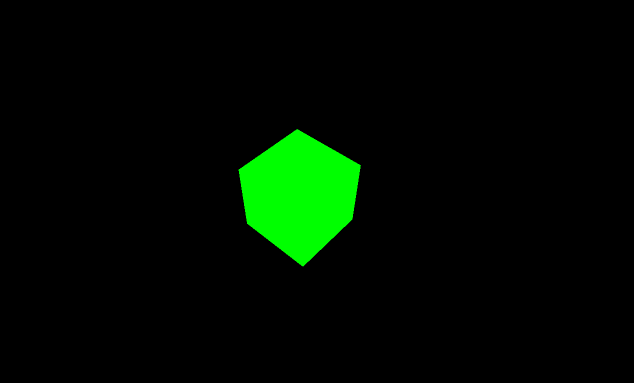
\includegraphics[width=8cm, height=8cm]{example1.png}
    \caption{First example: cube rotating.}
    \label{fig:firstcube}
\end{figure}

\section{Visualization of a polygonal mesh with color}

First, we will work on some 2D primitives. We will modify the previous example to visualize a black 2D triangle. Use the following coordinates for the vertices (-1,-1,0) (1,-1,0) and (1,1,0). We add the following code:

\begin{lstlisting}[language=JavaScript, caption=2D Primitives.]

			// geometry
            var geometry = new THREE.BufferGeometry();

            // attributes
            const vertices = new Float32Array( [
                -1.0, -1.0,  0.0,
                1.0, -1.0,  0.0,
                1.0,  1.0,  0.0,

            // 3 vertices per point
            geometry.setAttribute( 'position', new THREE.BufferAttribute( vertices, 3 ) );
            ] );

\end{lstlisting}

Here we defined the geometry, as well as the position of the vertices of our triangle. 
What we want to do next is to change the color of the triangle, as well as the color of the background. To do this we alter the \textbf{material} constant to change the color of the triangle to black, with the color attribute \textit{0x11111}. To add the background color red, we add the function \textbf{.setClearColor}\textit{(0xb20000)} when rendering, with what is inside the parentheses being the color attribute for the chosen red. Everything else remains the same as in the previous example, as we can see here:
\begin{lstlisting}[language=JavaScript, caption=2D Primitives and color.]
             // geometry
            var geometry = new THREE.BufferGeometry();

            // attributes
            const vertices = new Float32Array( [
                -1.0, -1.0,  0.0,
                1.0, -1.0,  0.0,
                1.0,  1.0,  0.0,
            ] );


            // 3 vertices per point
            geometry.setAttribute( 'position', new THREE.BufferAttribute( vertices, 3 ) );
            
            // material 
            const material = new THREE.MeshBasicMaterial( { color: 0x111111 } );
            
            // figure
            const triangle = new THREE.Mesh( geometry, material );
            scene.add( triangle );

            // set background color 
            renderer.setClearColor( 0xb20000);

			function animate() {
				requestAnimationFrame( animate );

				//cube.rotation.x += 0.01;
				//cube.rotation.y += 0.01;

				renderer.render( scene, camera );
			};

			animate();



			 camera.position.z = 5;

\end{lstlisting}

We got the expected output as we can see in the screenshot represented in \hyperref[fig:2dprimitives]{Fig.2}.

\begin{figure}[H]
    \centering
    
\includegraphics[width=8cm, height=8cm]{2dprimitives.png}
    \caption{2D primitives and color.}
    \label{fig:2dprimitives}
\end{figure}

The file for this output is called \textit{2D$_$primitives$_$colors.html} and can be found on the folder \textit{visualizationofapolygonalmeshwithcolor}.\\

In the next step, we played a little bit with colors,  by mapping different colors in a mesh face, it is necessary to associate a color to each vertice. Besides that, we also change the code for the \textbf{material}, as we can see below. The rest of the code remains the same.

\begin{lstlisting}[language=JavaScript, caption=2D Mapping colors.]
           // adding color to each vertice
            var colors = new Uint8Array( [
                255,  0,  0,  
                0,  255,  0,  
                0,  0,  255,  
            ] );

            geometry.setAttribute( 'color', new THREE.BufferAttribute( colors, 3, true) );
            
            // material 
            const material = new THREE.MeshBasicMaterial( {vertexColors: true} );
            
            // figure
            const triangle = new THREE.Mesh( geometry, material );
            scene.add( triangle );

			function animate() {
				requestAnimationFrame( animate );

				//cube.rotation.x += 0.01;
				//cube.rotation.y += 0.01;

				renderer.render( scene, camera );
			};

			animate();


			 camera.position.z = 5;
\end{lstlisting}
        
Now, we can see the output was the expected, as we can see in \hyperref[fig:mappingcolor]{Fig.3}.

\begin{figure}[H]
    \centering
    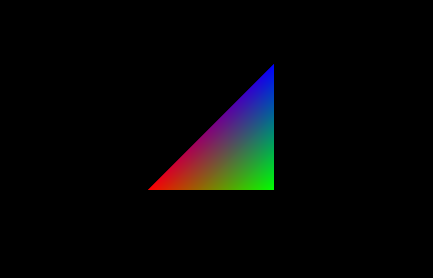
\includegraphics[width=8cm, height=8cm]{mappingcolor.png}
    \caption{Mapping color.}
    \label{fig:mappingcolor}
\end{figure}

The file for this output is called \textit{additionofcolor$_$1triangle} and can be found on the same folder as the previous one. \\

To finish this section, we created multiple triangles, with multiple colors, including the last one we created. 
To do this, we assigned 4 different geometries for the 4 different triangles we wanted to create: 

\begin{lstlisting}[language=JavaScript, caption=Geometries.]
          // geometry
        var geometry1 = new THREE.BufferGeometry();
        var geometry2 = new THREE.BufferGeometry();
        var geometry3 = new THREE.BufferGeometry();
        var geometry4 = new THREE.BufferGeometry();

\end{lstlisting}

Now, to actually position our triangles we had to assign the position to each one of them and set it to each one of the geometries.

\begin{lstlisting}[language=JavaScript, caption=Position.]
          // attributes
		// triang1
        const vertices1 = new Float32Array([
            0.0, 0.0, 0.0,
            0.5, 0.75, 0.0,
            1.0, 0.0, 0.0,
        ]);

		// triang2
        const vertices2 = new Float32Array([
            0.0, 0.0, 0.0,
            -0.35, -1.0, 0.0,
            -0.7, 0.25, 0.0,
        ]);

		// triang3
        const vertices3 = new Float32Array([
            -0.2, 0.15, 0.0,
            0.35, 0.65, 0.0,
            -0.85, 0.9, 0.0,
        ]);

		// triang4
        const vertices4 = new Float32Array([
            0.15, -0.95, 0.0,
            0.90, -0.7, 0.0,
            0.65, 0.10, 0.0,
        ]);


        // 3 vertices per point
        geometry1.setAttribute('position', new THREE.BufferAttribute(vertices1, 3));
        geometry2.setAttribute('position', new THREE.BufferAttribute(vertices2, 3));
        geometry3.setAttribute('position', new THREE.BufferAttribute(vertices3, 3));
        geometry4.setAttribute('position', new THREE.BufferAttribute(vertices4, 3));
\end{lstlisting}

We add the color just like in the previous example, which is, we assign a color to each vertice of the triangle. For triangles that only had one color, we added the same color to each vertice so it stayed uniform. We add also the colors to the \textbf{material}.  To be able to see all the triangles, also have to use the "side" flag in the \textbf{material} with the argument \textbf{THREE.DoubleSide}. This issue is related to the fact that only triangles with normal facing towards the camera are rendered.

\begin{lstlisting}[language=JavaScript, caption=Setting color.]
         // adding color to each vertice
        var colors = new Uint8Array([
            255, 0, 255,
            255, 0, 255,
            255, 0, 255,
        ]);
        var colors2 = new Uint8Array([
            255, 255, 0,
            255, 255, 0,
            255, 255, 0,
        ]);

        var colors3 = new Uint8Array([
            255, 0, 0,
            0, 255, 0,
            0, 0, 255,
        ]);
        var colors4 = new Uint8Array([
            0, 0, 0,
            0, 0, 0,
            0, 0, 0,
        ]);
        
        geometry1.setAttribute('color', new THREE.BufferAttribute(colors, 3, true));
        geometry2.setAttribute('color', new THREE.BufferAttribute(colors2, 3, true));
        geometry3.setAttribute('color', new THREE.BufferAttribute(colors3, 3, true));
        geometry4.setAttribute('color', new THREE.BufferAttribute(colors4, 3, true));

        // material
        const material1 = new THREE.MeshBasicMaterial({ vertexColors: true, side: THREE.DoubleSide });
        const material2 = new THREE.MeshBasicMaterial({ vertexColors: true, side: THREE.DoubleSide });
        const material3 = new THREE.MeshBasicMaterial({ vertexColors: true, side: THREE.DoubleSide });

		// figure
        const triangle1 = new THREE.Mesh(geometry1, material1);
        const triangle2 = new THREE.Mesh(geometry2, material2);
        const triangle3 = new THREE.Mesh(geometry3, material3);
\end{lstlisting}

Regarding the last triangle, since we want a transparent triangle with a white border, let's define the limits of the triangle and set its color to white (\textit{0xffffffff}), then add it to the scene.


\begin{lstlisting}[language=JavaScript, caption=Define edges.]
        // define white edges for the 4th triangle
		const edges = new THREE.EdgesGeometry( geometry4 );
		const line = new THREE.LineSegments( edges, new THREE.LineBasicMaterial( { color: 0xffffff } ) );


        scene.add(triangle1);
        scene.add(triangle2);
        scene.add(triangle3);
        scene.add(line);

        function animate() {
            requestAnimationFrame(animate);
            renderer.render(scene, camera);
        };

        animate();


        camera.position.z = 5;
\end{lstlisting}

So we managed to get a pretty accurate duplicate of the desired image, as we can see in \hyperref[fig:multiple]{Fig.4}

\begin{figure}[H]
    \centering
    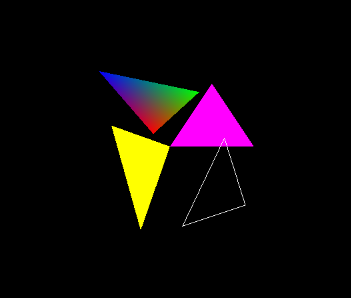
\includegraphics[width=8cm, height=8cm]{multiple.png}
    \caption{Multiple Polygons.}
    \label{fig:multiple}
\end{figure}

The file to get this output is called \textit{aditionofcolor$_$4triangles.html} and, again, on the same folder as before.

\section{Viewport Update}
Now, we will go back to the first example (rotation cube). Changing the dimensions of the browser window we can see that the visualization window (viewport) is not updated when the browser window size changes. To solve this problem, we create a new function to be called when the browser window size is updated. This function needs to access the window size (\textbf{window.innerWidth} and \textbf{window.innerHeight}) and update the renderer size accordingly (\textbf{renderer.setSize()}). We also need to modify the aspect camera ratio as well (\textbf{camera.aspect=…}) and update this change (\textbf{camera.updateProjectionMatrix()}), as we can see in the code bellow: 
\begin{lstlisting}[language=JavaScript, caption=Viewport update.]
        // viewport_update
            window.addEventListener('resize', function( )
            {
                var width = window.innerWidth;
                var height = window.innerHeight;
                renderer.setSize(width,height);
                camera.aspect = width/height;
                camera.updateProjectionMatrix( );
            });
\end{lstlisting}
The rest of the code stays the same. 
So we can see by the following screenshot that the viewport size was shrunk but the image updated to its position:

\begin{figure}[H]
    \centering
    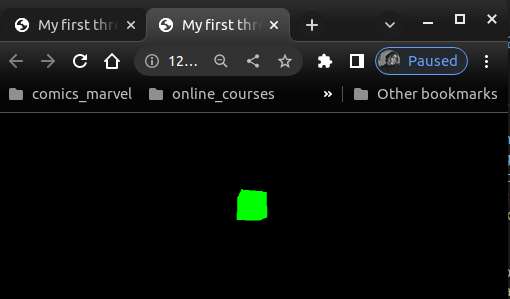
\includegraphics[width=8cm, height=8cm]{viewport.png}
    \caption{Viewport Update.}
    \label{fig:viewport}
\end{figure}

This code is in the file \textit{viewport$_$update$_$firstexample.html} and on the folder \textit{viewportupdate}.

\section{Other primitives in \textit{three.js}}
We modified the first example to show the cube in the wireframe. To do that we just have to set the \textbf{wideframe} to \textbf{true} on the \textbf{material}:

\begin{lstlisting}[language=JavaScript, caption=Wireframe.]
       const geometry = new THREE.BoxGeometry( 1, 1, 1 );
			const material = new THREE.MeshBasicMaterial( { color: 0x00ff00, wireframe: true} );
			const cube = new THREE.Mesh( geometry, material );
			scene.add( cube );
            });
\end{lstlisting}

So we can see a screenshot of our output in \hyperref[fig:wireframe]{Fig.6}.
\begin{figure}[H]
    \centering
    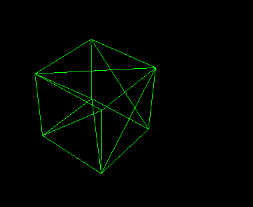
\includegraphics[width=8cm, height=8cm]{wireframe.png}
    \caption{Wireframe.}
    \label{fig:wireframe}
\end{figure}

The code for this is in the file \textit{firstexample$_$wireframe.html} on the folder \textit{Otherprimitives}.
 
 
 To finish this assignment, we investigated other available geometries and visualize at least 4 other geometries in the same scene changing some of their default parameters, like size or color. 
 We can see our different outputs here: 
 \begin{figure}[H]
    \centering
    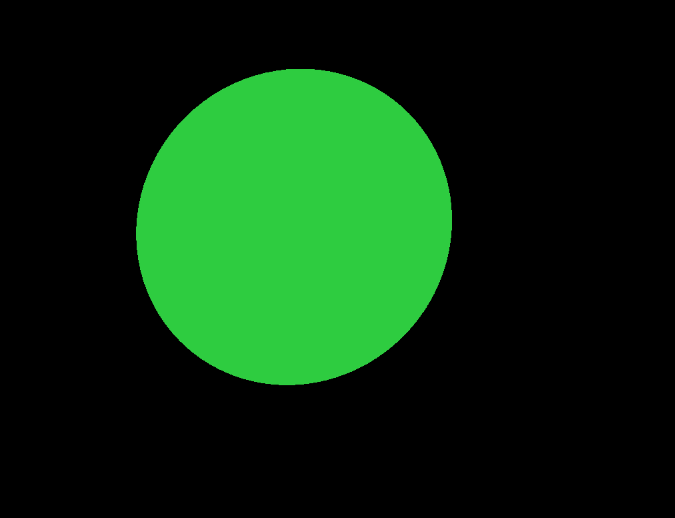
\includegraphics[width=8cm, height=8cm]{circle.png}
    \caption{Circle.}
    \label{fig:circle}
\end{figure}
\begin{figure}[H]
    \centering
    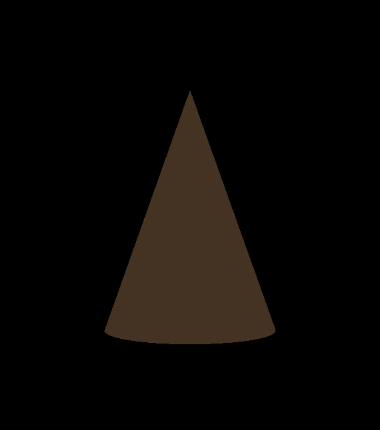
\includegraphics[width=8cm, height=8cm]{cone.png}
    \caption{Cone.}
    \label{fig:cone}
\end{figure}
\begin{figure}[H]
    \centering
    
\includegraphics[width=8cm, height=8cm]{ring.png}
    \caption{Ring.}
    \label{fig:ring}
\end{figure}

The code for these files can be found in the folder \textit{Otherprimitives}. \\
Now for the last figure, we decided to apply a wireframe again but in a different way: 
\begin{lstlisting}[language=JavaScript, caption=Wireframe.]
      const geometry =  new THREE.SphereGeometry( 2, 2, 2 ); // changed default size
			const material =  new THREE.MeshBasicMaterial( { color: 0xff851b} ); // changed default color
			const sphere = new THREE.Mesh( geometry, material );
			scene.add( sphere );

            const wireframe = new THREE.WireframeGeometry( geometry );

            const line = new THREE.LineSegments( wireframe );
            line.material.depthTest = false;
            line.material.opacity = 1;
            line.material.transparent = true;

            scene.add( line );

			camera.position.z = 5;

			function animate() {
				requestAnimationFrame( animate );

				sphere.rotation.x += 0.01;
				sphere.rotation.y += 0.01;

				renderer.render( scene, camera );
			};

			animate();
\end{lstlisting}

So, as an output, we get a static wireframe and a rotating figure around this wireframe: 

\begin{figure}[H]
    \centering
    
\includegraphics[width=8cm, height=8cm]{pyramide.png}
    \caption{Wireframe2.}
    \label{fig:wireframe2}
\end{figure}

The code for this output can be found in the file \textit{WireframeGeometry$_$extra4.html} in the folder \textit{Otherprimitives}. \\
\\



\cite{classesgit} \cite{examples} \cite{learn}

% Bibliography
%--------------------
\bibliographystyle{plain} % We choose the "plain" reference style
\bibliography{sources} % Entries are in the refs.bib file

\end{document}
